\documentclass{article}


\usepackage{arxiv}

\usepackage[utf8]{luainputenc}	% allow utf-8 input with LuaLaTeX
\usepackage[T1]{fontenc}    	% use 8-bit T1 fonts
\usepackage{palatino}			% use palatino font
\usepackage{hyperref}       	% hyperlinks
\usepackage{url}            	% simple URL typesetting
\usepackage{booktabs}       	% professional-quality tables
\usepackage{amsfonts}       	% blackboard math symbols
\usepackage{amsthm}
\usepackage{nicefrac}       	% compact symbols for 1/2, etc.
\usepackage{microtype}      	% microtypography
\usepackage{amsmath}
\usepackage[compat=1.1.0]{tikz-feynman}
\usepackage{tikz}
\usepackage{slashed}
\usepackage{mathtools}
\usepackage{dsfont}
\usepackage{geometry}
\usepackage{caption}
\usepackage[onehalfspacing]{setspace}



\numberwithin{equation}{section} % numbers equations by section

\newcommand{\Tr}{\mathrm{Tr}}
\newcommand{\fsl}{\slashed}
\newcommand{\lbr}{\left\lbrace}
\newcommand{\rbr}{\right\rbrace}
\newcommand*\circled[1]{\tikz[baseline=(char.base)]{
            \node[shape=circle,draw,inner sep=0.5pt] (char) {#1};}}
\newcommand\numberthis{\addtocounter{equation}{1}\tag{\theequation}}


\title{Contribution of QED to Rational Terms in 1-loop Feynman Diagrams in the Standard Model}




\author{
  Jonathan Kley \\
  Department of Physics\\
  Technical University of Munich\\
  James-Franck-Str. 1, 85748 Garching \\
  \texttt{jonathan.kley@tum.de} \\
}

\begin{document}

\maketitle

\begin{abstract}
The abstract goes here.
\end{abstract}


% keywords can be removed
\keywords{QFT \and 1-loop Feynman Diagrams \and Rational Terms \and More}

\newpage
\tableofcontents
\newpage

\section{Introduction}
\label{sec:Introduction} 

The introduction goes here.

\begin{equation}
\mathcal{M} = \sum_i d_i \mathrm{Box}_i + \sum_i c_i \mathrm{Triangle}_i + \sum_i b_i \mathrm{Bubble}_i + \sum_i a_i \mathrm{Tadpole}_i + R
\end{equation}

\begin{equation}
R = R_1 + R_2
\end{equation}
where $R_2$ is the $\epsilon$-dimensional contribution of dimensional regularization to the amplitude which is just a rational combination of Lorentz tensors and parameters of the theory, i.e. the couplings or masses of the particles in the theory.


We can decompose any m-point 1-loop function $\bar{A}\bar{q})$ in a numerator $\bar{N}( \bar{q})$ and denominators $\bar{D}_i$
\begin{equation}
\label{eqn:amp}
\bar{A} (\bar{q}) = \frac{\bar{N}(\bar{q})}{\bar{D}_0\bar{D}_1\cdots\bar{D}_{m-1}}, \qquad \bar{D}_i = \left( \bar{q} + \bar{p}_i \right)^2 - m_i^2, p_0 \neq 0
\end{equation}
where $\bar{q}$ is the $d$-dimensional loop momentum and $m_i$ is the mass of the particle corresponding to the propagator with the numerator $D_i$. The $d$-dimensional numerator function $\bar{N}(\bar{q})$ can be split in a 4-dimensional and an $\epsilon$-dimensional part 
\begin{equation}
\bar{N}( \bar{q}) = N (q) + \tilde{N} (\tilde{q}^2,q,\epsilon)
\end{equation}
where only $\tilde{N} (\tilde{q}^2,q,\epsilon)$ is interesting to us because it appears in the definitions of rational terms of the form $R_2$ which are defined as
\begin{equation}
R_2 \equiv \frac{1}{\left( 2\pi \right)^4} \int d^d \bar{q} \frac{\tilde{N} ( \tilde{q}^2,q,\epsilon)}{\bar{D}_0\bar{D}_1\cdots\bar{D}_{m-1}}
\end{equation}
which is the $\epsilon$-dimensional contribution to the amplitude in eqn. \ref{eqn:amp} integrated over the $d$-dimensional loop momentum $\bar{q}$. \\
To simplify our calculations later, we can establish a few identities for the manipulation of $d$-dimensional momenta.

e.g. in reference \cite{R2QCD} and \cite{R2QED}.




\section{R$_2$ in Pure QED}
\label{sec:pureQED} 
\subsection{2-point functions}
{\bf Photon self-energy} \\
\begin{align*}
\begin{gathered}
\feynmandiagram [layered layout, horizontal=b to c] {
	a [particle=\(\alpha\)] -- [photon, momentum=\(p_1\)] b
	  -- [fermion, half left, looseness=1.5, momentum=\(p_1+q\)] c
	  -- [fermion, half left, looseness=1.5, momentum=\(q\)] b,
	c -- [photon, momentum=\(p_1\)] d [particle=\(\beta\)] ,
};
\end{gathered} \qquad
& =\int\frac{d^dq}{\left( 2\pi \right)^d} \left( -1 \right) \mathrm{Tr} \lbr ie \gamma^{\alpha} \frac{i \left( \fsl{p}_1+\fsl{q}+m \right)}{\left( p_1+q \right)^2 - m^2} ie \gamma^{\beta} \frac{i \left( \fsl{q}+m \right)}{q^2 - m^2} \rbr & \\
& \equiv \int\frac{d^dq}{\left( 2\pi \right)^d} \frac{\bar{N}}{\bar{D}_1\bar{D}_0} &
\end{align*}

From now on bared quantities are $d$-dimensional, the quantities with a tilde $\epsilon$-dimensional and the normal momenta and gamma matrices 4-dimensional. 
\begin{equation*}
\bar{N} \left( \bar{q} \right) = - e^2 \ \mathrm{Tr} \lbr \bar{\gamma}^{\alpha} \left( \bar{\fsl{p}}_1 + \bar{\fsl{q}} + m \right) \bar{\gamma}^{\beta} \left( \bar{\fsl{q}} + m \right) \rbr = - e^2 \ \mathrm{Tr} \lbr \gamma^{\alpha} \left( \fsl{p}_1 + \fsl{q} + m \right) \gamma^{\beta} \left( \fsl{q} + m \right) + \gamma^{\alpha} \tilde{\fsl{q}} \gamma^{\beta} \tilde{\fsl{q}} \rbr \equiv N + \tilde{N}
\end{equation*}

\begin{equation*}
\tilde{N} = -e^2 \ \mathrm{Tr} \lbr \gamma^{\alpha} \tilde{\fsl{q}} \gamma^{\beta} \tilde{\fsl{q}} \rbr \overset{\left\lbrace \gamma^{\mu} , \tilde{\gamma}^{\nu} \right\rbrace = 0}{=} 4 e^2 \tilde{q}^2 g^{\alpha\beta}
\end{equation*}

\begin{equation}
\label{eqn:R2photon}
R_2^{\gamma\gamma} = \frac{1}{\left( 2\pi \right) ^4} \int d^d\bar{q} \frac{\tilde{N}}{\bar{D}_1\bar{D}_0} = \frac{4e^2}{16\pi^4} \underbrace{\int d^d\bar{q} \frac{\tilde{q}^2}{\bar{D}_1\bar{D}_0}}_{-i\frac{\pi}{2} \left( m^2 - p_1^2/3 \right)} = \frac{-ie^2}{8\pi^2} g^{\alpha\beta} \left( 2m^2 -\frac{p_1^2}{3} \right)
\end{equation}
\\

{\bf Electron self-energy} \\
\begin{align*}
\begin{gathered}
\feynmandiagram [layered layout, horizontal=b to c] {
	a -- [fermion, momentum=\(p_1\)] b,
	c -- [photon, half left, looseness=1.5, momentum=\(q\)] b,
	b -- [fermion, momentum=\(p_1+q\)] c,
	c -- [fermion, momentum=\(p_1\)] d,
};
\end{gathered} \qquad
& =\int\frac{d^dq}{\left( 2\pi \right)^d} ie \gamma^{\alpha} \frac{i \left( \fsl{p}_1+\fsl{q}+m \right)}{\left( p_1+q \right)^2 - m^2} ie \gamma^{\beta} \frac{-i g_{\alpha\beta}}{q^2} =\int\frac{d^dq}{\left( 2\pi \right)^d} \left( -e^2 \right) \gamma^{\alpha} \frac{\left( \fsl{p}_1+\fsl{q}+m \right)}{\left( p_1+q \right)^2 - m^2} \gamma_{\alpha} \frac{1}{q^2} & \\
& \equiv \int\frac{d^dq}{\left( 2\pi \right)^d} \frac{\bar{N}}{\bar{D}_1\bar{D}_0} &
\end{align*}

\begin{equation*}
\bar{N} \left( \bar{q} \right) = \left( -e^2 \right) \bar{\gamma}^{\alpha} \left( \bar{\fsl{p}}_1 + \bar{\fsl{q}} + m \right) \bar{\gamma}_{\alpha} = -e^2 \lbr \gamma^{\alpha} \left( \bar{\fsl{p}}_1 + \bar{\fsl{q}} + m \right) \gamma_{\alpha} + \tilde{\gamma}^{\alpha} \left( \bar{\fsl{p}}_1 + \bar{\fsl{q}} + m \right) \tilde{\gamma}_{\alpha} + \gamma^{\alpha} \tilde{\fsl{q}} \gamma_{\alpha} + \tilde{\gamma}^{\alpha} \tilde{\fsl{q}} \tilde{\gamma}_{\alpha} \rbr \equiv N + \tilde{N}
\end{equation*}

\begin{equation*}
\tilde{N} = -e^2 \lbr \tilde{\gamma}^{\alpha} \left( \bar{\fsl{p}}_1 + \bar{\fsl{q}} + m \right) \tilde{\gamma}_{\alpha} + \gamma^{\alpha} \tilde{\fsl{q}} \gamma_{\alpha} + \tilde{\gamma}^{\alpha} \tilde{\fsl{q}} \tilde{\gamma}_{\alpha} \rbr = -e^2 \lbr - \underbrace{\tilde{\gamma}^{\alpha} \tilde{\gamma}_{\alpha}}_{= \epsilon} \left( \bar{\fsl{p}}_1 + \bar{\fsl{q}} - m \right) - \underbrace{\gamma^{\alpha} \gamma_{\alpha}}_{=4} \tilde{\fsl{q}} + \tilde{\gamma}^{\alpha} \tilde{\fsl{q}} \tilde{\gamma}_{\alpha} \rbr
\end{equation*}
\begin{align*}
R_2^{\mathrm{ee}} & = \frac{1}{\left( 2\pi \right) ^4} \int d^d\bar{q} \frac{\tilde{N}}{\bar{D}_1\bar{D}_0} = \frac{-e^2}{\left( 2\pi \right) ^4} \int d^d\bar{q} \frac{1}{\bar{D}_1\bar{D}_0} \left( -\epsilon \left( \fsl{p}_1 + \fsl{q} - m \right) + \underbrace{\tilde{\fsl{q}} \left( \ldots \right)}_{=0} \right) = & \\ 
& = \frac{e^2}{\left( 2\pi \right) ^4} \lbr \underbrace{\int d^d\bar{q} \frac{\epsilon \left( \fsl{p}_1 - m \right)}{\bar{D}_1\bar{D}_0}}_{=-2\epsilon \frac{i \pi^2}{\epsilon}  \left( \fsl{p}_1 -m \right)}  + \underbrace{\int d^d\bar{q} \frac{\epsilon \fsl{q}}{\bar{D}_1\bar{D}_0}}_{=\epsilon \frac{i\pi^2}{\epsilon} \fsl{p}_1} \rbr = \frac{e^2}{\left( 2\pi \right) ^4} \epsilon \frac{i\pi^2}{\epsilon} \left( \left( -2 \right) \left( \fsl{p}_1 - m \right) + \fsl{p}_1 \right) = \frac{-ie^2}{16 \pi^2}  \left( \fsl{p}_1 - 2m \right) & \numberthis \label{eqn:R2ee}
\end{align*}


\subsection{3-point function}
\begin{align*}
\begin{gathered}
\feynmandiagram [horizontal=i1 to v2] {
	i1 [particle=\mu] -- [photon, momentum=\(p_2-p_1\)] v2,
	f1 -- [fermion, momentum=\(p_1\)] v1
	   -- [fermion, momentum=\(p_1+q\)] v2
	   -- [fermion, momentum=\(p_2+q\)] v3
	   -- [fermion, momentum=\(p_2\)] f3,
	v3 -- [boson, momentum=\(q\)] v1, 
};
\end{gathered} \qquad
& =\int\frac{d^dq}{\left( 2\pi \right)^d} ie \gamma^{\beta} \frac{i \left( \fsl{p}_1+\fsl{q}+m \right)}{\left( p_1+q \right)^2 - m^2} ie \gamma^{\mu} \frac{i \left( \fsl{p}_2 + \fsl{q}+m \right)}{\left( p_2 + q \right)^2 - m^2} ie \gamma^{\alpha} \frac{-ig_{\alpha\beta}}{q^2} & \\
& \equiv \int\frac{d^dq}{\left( 2\pi \right)^d} \frac{\bar{N}}{\bar{D}_1\bar{D}_2\bar{D}_0} &
\end{align*}

\begin{align*}
\bar{N} \left( \bar{q} \right) & = e^3 \lbr \bar{\gamma}^{\beta} \left( \bar{\fsl{p}}_1 + \bar{\fsl{q}} + m \right) \bar{\gamma}^{\mu} \left( \bar{\fsl{p}}_2 + \bar{\fsl{q}} + m \right) \bar{\gamma}_{\beta} \rbr = e^3 \lbr \gamma^{\beta} \left( \fsl{p}_1 + \fsl{q} + m \right) \gamma^{\mu} \left( \fsl{p}_2 + \fsl{q} + m \right) \gamma_{\beta} + \right. & \\
& \left. + \tilde{\gamma}^{\beta} \left( \fsl{p}_1 + \fsl{q} + m \right) \gamma^{\mu} \left( \fsl{p}_2 + \fsl{q} + m \right) \tilde{\gamma}_{\beta} + \underbrace{\gamma^{\beta} \tilde{\fsl{q}} \gamma^{\mu} \tilde{\fsl{q}} \gamma_{\beta}}_{\equiv \ \circled{1}} + \underbrace{\tilde{\gamma}^{\beta} \tilde{\fsl{q}} \gamma^{\mu} \tilde{\fsl{q}} \tilde{\gamma}_{\beta}}_{\equiv \ \circled{2}}  \rbr \equiv N + \tilde{N} &
\end{align*}
\begin{equation*}
\circled{1} = \tilde{q}_{\rho}\tilde{q}_{\sigma} \gamma^{\beta} \tilde{\gamma}^{\rho} \gamma^{\mu} \tilde{\gamma}^{\sigma} \gamma_{\beta} = \tilde{q}_{\rho}\tilde{q}_{\sigma} \left( -1 \right)^3 \tilde{\gamma}^{\rho} \tilde{\gamma}^{\sigma} \gamma^{\beta} \gamma^{\mu} \gamma_{\beta} = -2\tilde{\fsl{q}}\tilde{\fsl{q}}\gamma^{\mu} = -2 \tilde{q}^2 \gamma^{\mu}
\end{equation*}
\begin{equation*}
\circled{2} = \tilde{q}_{\rho}\tilde{q}_{\sigma} \tilde{\gamma}^{\beta} \tilde{\gamma}^{\rho} \gamma^{\mu} \tilde{\gamma}^{\sigma} \tilde{\gamma}_{\beta} = \tilde{q}_{\rho}\tilde{q}_{\sigma} \left( -1 \right)^2 \gamma^{\mu} \tilde{\gamma}^{\beta} \tilde{\gamma}^{\rho} \tilde{\gamma}^{\sigma} \tilde{\gamma}_{\beta} = \tilde{q}^2 \gamma^{\mu} \tilde{\gamma}^{\beta} \tilde{\gamma}_{\beta} = \epsilon \tilde{q}^2 \gamma^{\mu}
\end{equation*}

\begin{equation*}
\tilde{N} = - \epsilon \left( \fsl{p}_1 + \fsl{q} - m \right) \gamma^{\mu} \left( \fsl{p}_2 + \fsl{q} - m \right) - \left( 2 - \epsilon \right) \tilde{q}^2 \gamma^{\mu}
\end{equation*}
\begin{align*}
R_2^{\gamma\mathrm{ee}} = & \frac{1}{\left( 2\pi \right) ^4} \int d^d\bar{q} \frac{\tilde{N}}{\bar{D}_0 \bar{D}_1 \bar{D}_2} = \frac{1}{\left( 2\pi \right) ^4} \int d^d\bar{q} \frac{e^3}{\bar{D}_0 \bar{D}_1 \bar{D}_2} \lbr -\epsilon \left( \fsl{p}_1 + \fsl{q} - m \right) \gamma^{\mu} \left( \fsl{p}_2 + \fsl{q} - m \right) - \left( 2 - \epsilon \right) \tilde{q}^2 \gamma^{\mu} \rbr = & \\
& = \frac{e^3}{\left( 2\pi \right) ^4} \int d^d\bar{q} \frac{1}{\bar{D}_0 \bar{D}_1 \bar{D}_2} \lbr -\epsilon \fsl{q}\gamma^{\mu}\fsl{q} - \left( 2 - \epsilon \right) \tilde{q}^2 \gamma^{\mu} \rbr = \frac{e^3}{\left( 2\pi \right) ^4} \lbr -\epsilon \gamma^{\alpha}\gamma^{\mu}\gamma^{\beta} \left( \frac{-i\pi^2}{2\epsilon} g_{\alpha\beta} \right) - \frac{-i\pi^2}{2} \left(2 - \epsilon \right) \gamma^{\mu} \rbr = & \\
& = \frac{e^3}{\left( 2\pi \right) ^4} \frac{i \pi^2}{2} \lbr \gamma^{\alpha}\gamma^{\mu}\gamma_{\alpha} - 2\gamma^{\mu} + O(\epsilon) \rbr = \frac{-ie^3}{8\pi^2} \gamma^{\mu} & \numberthis \label{eqn:R2photonee}
\end{align*}

All other possible 3-pt. functions do not contribute to $R_2$ in QED. For example, (do triangle diagram)

\subsection{4-point function}
For the 4-point function we have to be more careful. The 1PI contribution at the 1-loop level consists of several diagrams. They are obtained by symmetrizing the external momenta of the diagram as follows
 \begin{align*}
\begin{gathered}
\feynmandiagram [small, horizontal=i1 to i2] {
	i4 [particle=\delta] -- [photon, momentum=\(p_2\)] v [crossed dot],
	i2 [particle=\beta] -- [photon, momentum=\(p_3\)] v,
	i1 [particle=\alpha] -- [photon, momentum=\(p_1\)] v,
	i3 [particle=\gamma] -- [photon, momentum=\(p_4\)] v,
};
\end{gathered}
= 2 \times \lbr
\begin{gathered}
\feynmandiagram [horizontal=i4 to i3] {
	i2 [particle=\beta] -- [photon, momentum=\(p_3\)] v2,
	i4 [particle=\delta] -- [photon, momentum=\(p_2\)] v4,
	i1 [particle=\alpha] -- [photon, momentum=\(p_1\)] v1,
	i3 [particle=\gamma] -- [photon, momentum=\(p_4\)] v3,
	v4 -- [fermion, momentum=\(q\)] v1
	   -- [fermion, momentum=\(p_1+q\)] v2
	   -- [fermion, momentum=\(q+p_1+p_3\)] v3
	   -- [fermion, momentum=\(q-p_2\)] v4,
};
\end{gathered}
\ \ + \ \ \left( \alpha \leftrightarrow \beta; \ p_1 \leftrightarrow p_3 \right) \ + \ \left( \alpha \leftrightarrow \delta; \ p_1 \leftrightarrow p_2 \right) \rbr 
\end{align*}

We only calculate one of the diagrams and do the symmetrizing with the result of our calculation, so we only have to evaluate one diagram. The first of the three diagrams gives
\begin{align*}
\begin{gathered}
\feynmandiagram [horizontal=i4 to i3] {
	i2 [particle=\beta] -- [photon, momentum=\(p_3\)] v2,
	i4 [particle=\delta] -- [photon, momentum=\(p_2\)] v4,
	i1 [particle=\alpha] -- [photon, momentum=\(p_1\)] v1,
	i3 [particle=\gamma] -- [photon, momentum=\(p_4\)] v3,
	v4 -- [fermion, momentum=\(q\)] v1
	   -- [fermion, momentum=\(p_1+q\)] v2
	   -- [fermion, momentum=\(q+p_1+p_3\)] v3
	   -- [fermion, momentum=\(q-p_2\)] v4,
};
\end{gathered}\qquad
& = \int\frac{d^dq}{\left( 2\pi \right)^d} \left( -1 \right) \mathrm{Tr} \lbr ie \gamma^{\alpha} \frac{i \left( \fsl{p}_1 + \fsl{q} + m \right)}{\left( p_1 +q \right) ^2 -m^2} ie \gamma^{\beta} \frac{i \left( \fsl{q} + \fsl{p}_3 + \fsl{p}_1 + m \right)}{\left( p_3 + p_1 +q \right) ^2 -m^2} \times \right. & \\
& \left. \times ie \gamma^{\gamma} \frac{i \left( \fsl{q} - \fsl{p}_2 + m \right)}{\left( q - p_2 \right) ^2 - m^2} ie \gamma^{\delta} \frac{i \left( \fsl{q} + m \right)}{q ^2 - m^2} \rbr \equiv \int\frac{d^dq}{\left( 2\pi \right)^d} \frac{\bar{N}}{\bar{D}_1\bar{D}_{13}\bar{D}_2\bar{D}_0} &
\end{align*}

\begin{align*}
\bar{N} \left( \bar{q} \right) & = -e^4 \mathrm{Tr} \lbr \bar{\gamma}^{\alpha} \left( \bar{\fsl{p}}_1 + \bar{\fsl{q}} + m \right) \bar{\gamma}^{\beta} \left( \bar{\fsl{q}} +  \bar{\fsl{p}}_1 + \bar{\fsl{p}}_3 + m \right) \bar{\gamma}^{\gamma} \left( \bar{\fsl{q}} - \bar{\fsl{p}}_2 + m \right) \bar{\gamma}^{\delta} \left( \bar{\fsl{q}} + m \right) \rbr = & \\
& = -e^4 \mathrm{Tr} \lbr \gamma^{\alpha} \left( \fsl{p}_1 + \fsl{q} + m \right) \gamma^{\beta} \left( \fsl{q} +  \fsl{p}_1 + \fsl{p}_3 + m \right) \gamma^{\gamma} \left( \fsl{q} - \fsl{p}_2 + m \right) \gamma^{\delta} \left( \fsl{q} + m \right) + \right. &  \\
&  \left. + \gamma^{\alpha} \tilde{\fsl{q}} \gamma^{\beta} \tilde{\fsl{q}} \gamma^{\gamma} \tilde{\fsl{q}} \gamma^{\delta} \tilde{\fsl{q}} + \gamma^{\alpha} \tilde{\fsl{q}} \gamma^{\beta} \tilde{\fsl{q}} \gamma^{\gamma} \fsl{q} \gamma^{\delta} \fsl{q}  + \gamma^{\alpha} \fsl{q} \gamma^{\beta} \tilde{\fsl{q}} \gamma^{\gamma} \tilde{\fsl{q}} \gamma^{\delta} \fsl{q} + \gamma^{\alpha} \fsl{q} \gamma^{\beta} \fsl{q} \gamma^{\gamma} \tilde{\fsl{q}} \gamma^{\delta} \tilde{\fsl{q}} + \gamma^{\alpha} \tilde{\fsl{q}} \gamma^{\beta} \fsl{q} \gamma^{\gamma} \fsl{q} \gamma^{\delta} \tilde{\fsl{q}} + \right. & \\
& \left. + \gamma^{\alpha} \tilde{\fsl{q}} \gamma^{\beta} \fsl{q} \gamma^{\gamma} \tilde{\fsl{q}} \gamma^{\delta} \fsl{q} + \gamma^{\alpha} \fsl{q} \gamma^{\beta} \tilde{\fsl{q}} \gamma^{\gamma} \fsl{q} \gamma^{\delta} \tilde{\fsl{q}} \rbr \equiv N + \tilde{N} &
\end{align*}

Where we have used that the trace of an odd number of Dirac matrices is zero. Using (..) and (..) $\tilde{N}$ can be further simplified to
\begin{align*}
\tilde{N} = & -e^4 \mathrm{Tr} \lbr \left( -1 \right)^{10} \tilde{q}^4 \gamma^{\alpha} \gamma^{\beta} \gamma^{\gamma} \gamma^{\delta} + \tilde{q}^2 \left[ \left( -1 \right) ^3  \gamma^{\alpha} \gamma^{\beta} \gamma^{\gamma} \fsl{q} \gamma^{\delta} \fsl{q}  + \left( -1 \right)^7 \gamma^{\alpha} \fsl{q} \gamma^{\beta} \gamma^{\gamma} \gamma^{\delta} \fsl{q} + \left( -1 \right)^{11} \gamma^{\alpha} \fsl{q} \gamma^{\beta} \fsl{q} \gamma^{\gamma} \gamma^{\delta} + \right. \right. & \\
& \left. \left. + \left( -1 \right)^7 \gamma^{\alpha} \gamma^{\beta} \fsl{q} \gamma^{\gamma} \fsl{q} \gamma^{\delta} + \left( -1 \right)^5 \gamma^{\alpha} \gamma^{\beta} \fsl{q} \gamma^{\gamma} \gamma^{\delta} \fsl{q} + \left( -1 \right)^9 \gamma^{\alpha} \fsl{q} \gamma^{\beta} \gamma^{\gamma} \fsl{q} \gamma^{\delta} \right] \rbr = & \\
& = -e^4 \mathrm{Tr} \lbr \tilde{q}^4 \gamma^{\alpha} \gamma^{\beta} \gamma^{\gamma} \gamma^{\delta} - \tilde{q}^2 \left( \gamma^{\alpha} \gamma^{\beta} \gamma^{\gamma} \fsl{q} \gamma^{\delta} \fsl{q} + \gamma^{\alpha} \fsl{q} \gamma^{\beta} \gamma^{\gamma} \gamma^{\delta} \fsl{q} + \gamma^{\alpha} \fsl{q} \gamma^{\beta} \fsl{q} \gamma^{\gamma} \gamma^{\delta} + \gamma^{\alpha} \gamma^{\beta} \fsl{q} \gamma^{\gamma} \fsl{q} \gamma^{\delta} + \right. \right. & \\
& \left. \left. + \gamma^{\alpha} \gamma^{\beta} \fsl{q} \gamma^{\gamma} \gamma^{\delta} \fsl{q} + \gamma^{\alpha} \fsl{q} \gamma^{\beta} \gamma^{\gamma} \fsl{q} \gamma^{\delta} \right) \rbr \equiv N + \tilde{N} &
\end{align*}
Since this expression involves the trace over up to 6 Dirac matrices, the calculation is very cumbersome. Wcane can evaluate this expression with the help of the Mathematica package FeynCalc \cite{FeynCalc,FeynCalc2} 
\begin{figure}[h!]
  \begin{center}
    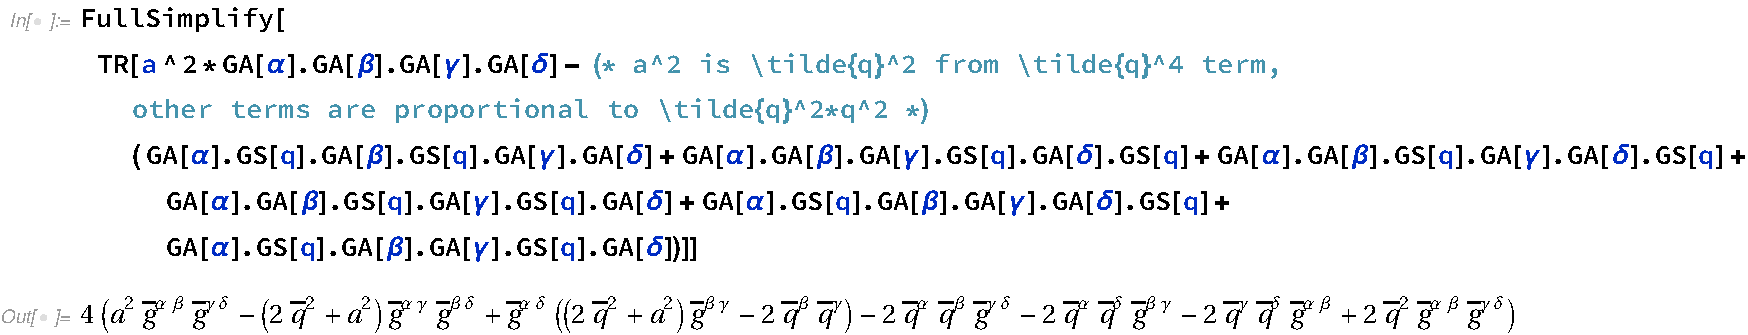
\includegraphics[width=1.0\textwidth]{Figures/Trace_4ptfct_Mathematica}
  \end{center}
  \setlength{\belowcaptionskip}{-20pt}
  \caption*{}
\end{figure} \\
As usual we plug this in the definition of $R_2$ and evaluate the integrals to get the expression of $R_2$ for the first of the contributing diagrams.
\begin{align*}
R_2 = & \frac{1}{\left( 2\pi \right) ^4} \int d^d\bar{q} \frac{\tilde{N}}{\bar{D}_0 \bar{D}_1 \bar{D}_2} = \frac{1}{\left( 2\pi \right) ^4} \int d^d\bar{q} \frac{4e^4}{\bar{D}_1 \bar{D}_{13} \bar{D}_2 \bar{0}} \tilde{q}^2 \lbr \left( 2q^2 + \tilde{q}^2 \right) \left( g^{\alpha\delta}g^{\beta\gamma} - g^{\alpha\gamma}g^{\beta\delta} + g^{\alpha\beta}g^{\gamma\delta} \right) + \right. & \\
& \left. - 2 \left( g^{\alpha\beta}q^{\gamma}q^{\delta} + g^{\gamma\delta}q^{\alpha}q^{\beta} + g^{\alpha\delta}q^{\beta}q^{\gamma} + g^{\beta\gamma}q^{\alpha}q^{\delta} \right) \rbr = & \\
& = \frac{-4e^4}{\left( 2\pi \right) ^4} \lbr \left( 2 \left( \frac{-i\pi^2}{3} \right) + \left( \frac{-i\pi^2}{6} \right) \right) \left( g^{\alpha\delta}g^{\beta\gamma} - g^{\alpha\gamma}g^{\beta\delta} + g^{\alpha\beta}g^{\gamma\delta} \right) - 2 \left( \frac{-i\pi^2}{12} \right) \left( g^{\alpha\beta}g^{\gamma\delta} + g^{\gamma\delta}g^{\alpha\beta} + \right. \right. & \\
& \left. \left. + g^{\alpha\delta}g^{\beta\gamma} + g^{\beta\gamma}g^{\alpha\delta} \right) \rbr = \frac{ie^4}{4\pi^2} \lbr \frac{5}{6} \left( g^{\alpha\delta}g^{\beta\gamma} - g^{\alpha\gamma}g^{\beta\delta} + g^{\alpha\beta}g^{\gamma\delta} \right) - \frac{1}{6} \left( 2 g^{\alpha\beta}g^{\gamma\delta} + 2g^{\alpha\delta}g^{\beta\gamma} +  \right) \rbr = & \\
& = \frac{ie^4}{24 \pi^2} \left( 3 g^{\alpha\beta}g^{\gamma\delta} - 5 g^{\alpha\gamma}g^{\beta\delta} + 3 g^{\beta\gamma}g^{\alpha\delta} \right) &
\end{align*}

\begin{align*}
R_2^{4\gamma} = & 2 \left( R_2 + R_2 \left( \alpha \leftrightarrow \delta \right) + R_2 \left( \alpha \leftrightarrow \beta \right) \right) = \frac{2ie^4}{24 \pi^2} \lbr \left( 3 g^{\alpha\beta}g^{\gamma\delta} - 5 g^{\alpha\gamma}g^{\beta\delta} + 3 g^{\beta\gamma}g^{\alpha\delta} \right) + \left( 3 g^{\beta\delta}g^{\alpha\gamma} - 5 g^{\gamma\delta}g^{\alpha\beta} + 3 g^{\beta\gamma}g^{\alpha\delta} \right) + \right. & \\
& \left. + \left( 3 g^{\alpha\beta}g^{\gamma\delta} - 5 g^{\beta\gamma}g^{\alpha\delta} + 3 g^{\alpha\gamma}g^{\beta\delta} \right) \rbr = \frac{ie^4}{12 \pi^2} \left( g^{\alpha\beta}g^{\gamma\delta} + g^{\alpha\gamma}g^{\beta\delta} + g^{\beta\gamma}g^{\alpha\delta} \right) & \numberthis \label{eqn:R24photon}
\end{align*}

All of the other 4-point functions vanish as well.
\section{QED Contribution to R$_2$ in the Standard Model}
\label{sec:QED2SM} 
\subsection{2-point functions}
{\bf Z-boson self-energy}
\begin{align*}
\begin{gathered}
\feynmandiagram [layered layout, horizontal=b to c] {
	a [particle={\(Z,\alpha\)}] -- [photon, momentum=\(p_1\)] b
	  -- [fermion, half left, looseness=1.5, momentum=\(p_1+q\)] c
	  -- [fermion, half left, looseness=1.5, momentum=\(q\)] b,
	c -- [photon, momentum=\(p_1\)] d [particle={\(\beta,Z\)}] ,
};
\end{gathered} \qquad
& =\int\frac{d^dq}{\left( 2\pi \right)^d} \left( -1 \right) \Tr \lbr \frac{ig}{cos\theta_W} \gamma^{\alpha} \left( g_V - g_A \gamma_5 \right) \frac{i \left( \fsl{p}_1+\fsl{q}+m \right)}{\left( p_1+q \right)^2 - m^2} \frac{ig}{cos\theta_W} \gamma^{\beta} \times \right. & \\
& \times \left. \left( g_V - g_A \gamma_5 \right) \frac{i \left( \fsl{q}+m \right)}{q^2 - m^2} \rbr = & \\
& =\int\frac{d^dq}{\left( 2\pi \right)^d} \frac{-g^2}{\cos^2\theta_W} \Tr \lbr \gamma^{\alpha} \left( g_V - g_A \gamma_5 \right) \frac{ \left( \fsl{p}_1+\fsl{q}+m \right)}{\left( p_1+q \right)^2 - m^2} \gamma^{\beta} \left( g_V - g_A \gamma_5 \right) \frac{ \left( \fsl{q}+m \right)}{q^2 - m^2} \rbr & \\
& \equiv \int\frac{d^dq}{\left( 2\pi \right)^d} \frac{\bar{N}}{\bar{D}_1\bar{D}_0} &
\end{align*}

Additionally to the four gamma matrices we now also have the fifth gamma matrix. Its extension to d dimensions is not as straightforward as with the four gamma matrices where we just have to change the 4-dimensional metric to the d-dimensional metric in the Clifford algebra $\lbr \gamma^{\alpha}, \gamma^{\beta} \rbr = 2 g^{\alpha\beta} $. This is because chirality is a property of four dimensions.\\
If we still want to impose $\lbr \gamma_5,\gamma^{\mu} \rbr = 0$, then $\Tr\left( \gamma_5 \gamma^{\alpha}\gamma^{\beta}\gamma^{\gamma}\gamma^{\delta} \right) = 0$  for $d \neq 0,2,4$ which clashes with $\Tr\left( \gamma_5 \gamma^{\alpha}\gamma^{\beta}\gamma^{\gamma}\gamma^{\delta} \right) = -4i \epsilon^{\alpha\beta\gamma\delta}$ \cite{Gamma5}. But the identity is essential in the evaluation of the triangle diagram for the Adler-Bell-Jackiw anomaly. The only definition of $\gamma_5$ which is consistent with the chiral anomaly is the definition of 't Hooft and Veltman \cite{HVgamma5}: $\gamma_5 = i/4! \ \epsilon_{\mu_1 \dots \mu_4} \gamma^{\mu_1} \cdots \gamma^{\mu_4}$. This definition implies $ \lbr \gamma_5, \gamma^{\mu} \rbr = 0 $ and $ \left[ \gamma_5, \tilde{\gamma}^{\mu} \right] = 0 $. 

\begin{align*}
\bar{N} \left( \bar{q} \right) = & - \frac{g^2}{\cos^2\theta_W} \ \Tr  \lbr \bar{\gamma}^{\alpha} \left( g_V - g_A \gamma_5 \right) \left( \bar{\fsl{p}}_1+\bar{\fsl{q}}+m \right) \bar{\gamma}^{\beta} \left( g_V - g_A \gamma_5 \right) \left( \bar{\fsl{q}}+m \right) \rbr = & \\
&= \frac{-g^2}{\cos^2\theta_W} \Tr \lbr \gamma^{\alpha} \left( g_V - g_A \gamma_5 \right) \left( \fsl{p}_1 + \fsl{q} + m \right) \gamma^{\beta} \left( g_V - g_A \gamma_5 \right) \left( \fsl{q} + m \right) + \gamma^{\alpha} \left( g_V^2 + g_A^2 \right) \tilde{\fsl{q}} \gamma^{\beta} \tilde{\fsl{q}} \rbr \equiv N + \tilde{N} &
\end{align*}
Where we used $ \left[ \gamma_5, \tilde{\gamma}^{\mu} \right] = 0 $ and the fact that the gamma matrices will be contracted with external momenta.
\begin{equation*}
\tilde{N} = \frac{-g^2}{\cos^2\theta_W} \left( g_V^2 + g_A^2 \right) \left( - \tilde{q}^2 \right) \Tr\left( \gamma^{\alpha}\gamma^{\beta} \right) = \frac{4g^2\tilde{q}^2}{\cos^2\theta_W} \left( g_V^2 + g_A^2 \right) g^{\alpha\beta}
\end{equation*}
\begin{align*}
R_2^{ZZ} & = \frac{1}{\left( 2\pi \right) ^4} \int d^d\bar{q} \frac{\tilde{N}}{\bar{D}_1\bar{D}_0} = \frac{4g^2g^{\alpha\beta}}{\left( 2\pi \right)^4 \cos^2\theta_W} \left( g_V^2 + g_A^2 \right) \int d^d\bar{q} \frac{\tilde{q}^2}{\bar{D}_1\bar{D}_0} = & \\
& = \frac{4g^2g^{\alpha\beta}}{\left( 2\pi \right)^4 \cos^2\theta_W} \left( g_V^2 + g_A^2 \right) \left( - \frac{i\pi^2}{2} \right) \left( m^2 - \frac{p_1^2}{3} \right) = \frac{-ig^2}{ 8 \pi^2 \cos^2\theta_W} \left( g_V^2 + g_A^2 \right)  \left( m^2 - \frac{p_1^2}{3} \right) g^{\alpha\beta} & \\ \numberthis \label{eqn:R2ZZ}
\end{align*}
\\

{\bf Photon/Z-boson mixed self-energy}
\begin{align*}
\begin{gathered}
\feynmandiagram [layered layout, horizontal=b to c] {
	a [particle={\(\gamma,\alpha\)}] -- [photon, momentum=\(p_1\)] b
	  -- [fermion, half left, looseness=1.5, momentum=\(p_1+q\)] c
	  -- [fermion, half left, looseness=1.5, momentum=\(q\)] b,
	c -- [photon, momentum=\(p_1\)] d [particle={\(\beta,Z\)}] ,
};
\end{gathered} \qquad
& =\int\frac{d^dq}{\left( 2\pi \right)^d} \left( -1 \right) \Tr \lbr \left( - i e Q_f \right) \gamma^{\alpha} \frac{i \left( \fsl{p}_1+\fsl{q}+m \right)}{\left( p_1+q \right)^2 - m^2} \frac{ig}{cos\theta_W} \gamma^{\beta} \times \right. & \\
& \times \left. \left( g_V - g_A \gamma_5 \right) \frac{i \left( \fsl{q}+m \right)}{q^2 - m^2} \rbr = & \\
& =\int\frac{d^dq}{\left( 2\pi \right)^d} \frac{eQ_fg}{\cos\theta_W} \Tr \lbr \gamma^{\alpha} \frac{ \left( \fsl{p}_1+\fsl{q}+m \right)}{\left( p_1+q \right)^2 - m^2} \gamma^{\beta} \left( g_V - g_A \gamma_5 \right) \frac{ \left( \fsl{q}+m \right)}{q^2 - m^2} \rbr & \\
& \equiv \int\frac{d^dq}{\left( 2\pi \right)^d} \frac{\bar{N}}{\bar{D}_1\bar{D}_0} &
\end{align*}

\begin{align*}
\bar{N} \left( \bar{q} \right) = & \frac{eQ_fg}{\cos\theta_W} \ \Tr \lbr \bar{\gamma}^{\alpha} \left( \bar{\fsl{p}}_1+\bar{\fsl{q}}+m \right) \bar{\gamma}^{\beta} \left( g_V - g_A \gamma_5 \right) \left( \bar{\fsl{q}}+m \right) \rbr = & \\
&= \frac{eQ_fg}{\cos\theta_W} \Tr \lbr \gamma^{\alpha} \left( \fsl{p}_1 + \fsl{q} + m \right) \gamma^{\beta} \left( g_V - g_A \gamma_5 \right) \left( \fsl{q} + m \right) + \gamma^{\alpha} \tilde{\fsl{q}} \gamma^{\beta} g_V \tilde{\fsl{q}} \rbr \equiv N + \tilde{N} &
\end{align*}
Where we have used $\Tr\left( \gamma^{\alpha}\gamma^{\beta}\gamma_5 \right) = 0$.

\begin{equation*}
\tilde{N} = \frac{eQ_fg}{cos\theta_W} \Tr\lbr \gamma^{\alpha} \tilde{\fsl{q}} \gamma^{\beta} g_V \tilde{\fsl{q}} \rbr = \frac{-4eQ_fgg_V}{\cos\theta_W} \tilde{q}^2 g^{\alpha\beta}
\end{equation*}

\begin{align*}
R_2^{\gamma Z} & = \frac{1}{\left( 2\pi \right)^4} \int d^d \bar{q} \frac{\tilde{N}}{\bar{D}_1\bar{D}_0} = \frac{-4eQ_fgg_V}{\left( 2\pi \right)^4\cos\theta_W} g^{\alpha\beta} \int d^d\bar{q} \frac{\tilde{q}^2}{\bar{D}_1\bar{D}_0} & \\
& = \frac{-4eQ_fgg_V}{\left( 2\pi \right)^4\cos\theta_W} \left( -\frac{i\pi^2}{2} \right) g^{\alpha\beta} \left( m^2 - \frac{p_1^2}{3} \right) = \frac{ieQ_fgg_V}{8\pi^2\cos\theta_W} g^{\alpha\beta} \left( m^2 - \frac{p_1^2}{3} \right) & \numberthis \label{eqn:R2photonZ}
\end{align*}

{\bf Gluon self-energy} \\
Because the gluon (just as the photon) couples to a pure vector current, the calculation for the gluon self-energy $R_2$ is the same as for the photon self-energy $R_2$ replacing the electric charge generator with the colour charge generator. So, from equation \ref{eqn:R2photon} with $e Q_f \rightarrow g_S T^a$ we get
\begin{equation}
\label{eqn:R2gluon}
R_2^{gg} = R_2^{\gamma\gamma} \left( e Q_f \rightarrow g_S T^a \right) = \frac{-ig_S^2}{8\pi^2} \Tr \left( T^a T^b \right) g^{\alpha\beta} \left( 2m^2 -\frac{p_1^2}{3} \right) 
\end{equation}

\subsection{3-point functions}
{\bf Gluon-quark vertex}
\begin{align*}
\begin{gathered}
\feynmandiagram [horizontal=i1 to v2] {
	i1 [particle=\(\mu\)] -- [gluon, momentum=\(p_2-p_1\)] v2,
	f1 -- [fermion, momentum=\(p_1\)] v1
	   -- [fermion, momentum=\(p_1+q\)] v2
	   -- [fermion, momentum=\(p_2+q\)] v3
	   -- [fermion, momentum=\(p_2\)] f3,
	v3 -- [boson, momentum=\(q\)] v1, 
};
\end{gathered} \qquad
& = \int\frac{d^dq}{\left( 2\pi \right)^d} \left( -ie Q_q \gamma^{\beta} \right) \frac{i \left( \fsl{p}_1+\fsl{q}+m \right)}{\left( p_1+q \right)^2 - m^2} \left( -ig_S \gamma^{\mu} T^a \right) \frac{i \left( \fsl{p}_2 + \fsl{q}+m \right)}{\left( p_2 + q \right)^2 - m^2} \left( -ie Q_q \gamma^{\alpha} \right) \frac{-ig_{\alpha\beta}}{q^2} = & \\
& = \int\frac{d^dq}{\left( 2\pi \right)^d} -e^2 Q_q^2 g_S \gamma^{\beta} \frac{ \left( \fsl{p}_1+\fsl{q}+m \right)}{\left( p_1+q \right)^2 - m^2} \gamma^{\mu} T^a \frac{ \left( \fsl{p}_2 + \fsl{q}+m \right) }{\left( p_2 + q \right)^2 - m^2} \gamma_{\beta} \frac{1}{q^2} = & \\
& \equiv \int\frac{d^dq}{\left( 2\pi \right)^d} \frac{\bar{N}}{\bar{D}_1\bar{D}_2\bar{D}_0} &
\end{align*}

\begin{align*}
\bar{N} \left( \bar{q} \right) & = -e^2 Q_q^2 g_S \lbr \bar{\gamma}^{\beta} \left( \bar{\fsl{p}}_1 + \bar{\fsl{q}} + m \right) \bar{\gamma}^{\mu} T^a \left( \bar{\fsl{p}}_2 + \bar{\fsl{q}} + m \right) \bar{\gamma}_{\beta} \rbr = -e^2 Q_q^2 g_S \lbr \gamma^{\beta} \left( \fsl{p}_1 + \fsl{q} + m \right) \gamma^{\mu} T^a \left( \fsl{p}_2 + \fsl{q} + m \right) \gamma_{\beta} + \right. & \\
& \left. + \gamma^{\beta} \tilde{\fsl{q}} \gamma^{\mu} T^a \tilde{\fsl{q}} \gamma_{\beta} + \tilde{\gamma}^{\beta} \fsl{q} \gamma^{\mu} T^a \fsl{q} \tilde{\gamma}_{\beta} \rbr \equiv N + \tilde{N} &
\end{align*}

\begin{equation*}
\tilde{N} = -e^2 Q_q^2 g_S \lbr -\tilde{q}^2 \underbrace{\gamma^{\beta}\gamma^{\mu}\gamma_{\beta}}_{-2\gamma^{\mu}} T^a - \epsilon q_{\alpha}q_{\beta} \gamma^{\alpha}\gamma^{\mu}\gamma^{\beta}  T^a \rbr = -e^2 Q_q^2 g_S \lbr 2\tilde{q}^2 \gamma^{\mu} T^a - \epsilon q_{\alpha}q_{\beta} \gamma^{\alpha}\gamma^{\mu}\gamma^{\beta} T^a \rbr
\end{equation*}

\begin{align*}
R_2^{gqq} = & \frac{1}{\left( 2\pi \right)^4} \int d^d \bar{q} \frac{\tilde{N}}{\bar{D}_1\bar{D}_2\bar{D}_0} = \frac{-e^2Q_q^2g_S}{\left( 2\pi \right)^4} \int d^d \bar{q} \frac{1}{\bar{D}_1\bar{D}_2\bar{D}_0} \lbr 2\tilde{q}^2 \gamma^{\mu} T^a - \epsilon q_{\alpha}q_{\beta} \gamma^{\alpha}\gamma^{\mu}\gamma^{\beta} T^a \rbr = & \\
& = \frac{-e^2Q_q^2g_S}{\left( 2\pi \right)^4} \lbr 2 \left( \frac{-i\pi^2}{2} \right) \gamma^{\mu} T^a - \epsilon \left( \frac{-i\pi^2}{2\epsilon} \right) \underbrace{g_{\alpha\beta} \gamma^{\alpha}\gamma^{\mu}\gamma^{\beta}}_{-2\gamma^{\mu}} T^a \rbr = \frac{-e^2 Q_q^2 g_S}{16 \pi^4} \left( \frac{-i\pi^2}{2} \right) \lbr 2\gamma^{\mu} T^a + 2\gamma^{\mu} T^a \rbr = & \\
& = \frac{ie^2 Q_q^2 g_S}{8 \pi^2} \gamma^{\mu} T^a & \numberthis \label{eqn:R2gluonqq}
\end{align*}


{\bf Z-fermion vertex}
\begin{align*}
\begin{gathered}
\feynmandiagram [horizontal=i1 to v2] {
	i1 [particle={\(Z,\mu\)}] -- [photon, momentum=\(p_2-p_1\)] v2,
	f1 -- [fermion, momentum=\(p_1\)] v1
	   -- [fermion, momentum=\(p_1+q\)] v2
	   -- [fermion, momentum=\(p_2+q\)] v3
	   -- [fermion, momentum=\(p_2\)] f3,
	v3 -- [boson, momentum=\(q\)] v1, 
};
\end{gathered} \qquad
& = \int\frac{d^dq}{\left( 2\pi \right)^d} \left( -ie Q_f \gamma^{\beta} \right) \frac{i \left( \fsl{p}_1+\fsl{q}+m \right)}{\left( p_1+q \right)^2 - m^2} \frac{ig}{\cos\theta_W} \gamma^{\mu} \left( g_V - g_A \gamma_5 \right) \frac{i \left( \fsl{p}_2 + \fsl{q}+m \right)}{\left( p_2 + q \right)^2 - m^2} \times & \\
& \times \left( -ie Q_f \gamma^{\alpha} \right) \frac{-ig_{\alpha\beta}}{q^2} = & \\
& = \int\frac{d^dq}{\left( 2\pi \right)^d} \frac{e^2 Q_f^2g}{\cos\theta_W} \gamma^{\beta} \frac{ \left( \fsl{p}_1+\fsl{q}+m \right)}{\left( p_1+q \right)^2 - m^2} \gamma^{\mu} \left( g_V - g_A \gamma_5 \right) \frac{ \left( \fsl{p}_2 + \fsl{q}+m \right) }{\left( p_2 + q \right)^2 - m^2} \gamma_{\beta} \frac{1}{q^2} = & \\
& \equiv \int\frac{d^dq}{\left( 2\pi \right)^d} \frac{\bar{N}}{\bar{D}_1\bar{D}_2\bar{D}_0} &
\end{align*}

\begin{align*}
\bar{N} \left( \bar{q} \right) & = \frac{e^2Q_f^2g}{\cos\theta_W} \lbr \bar{\gamma}^{\beta} \left( \bar{\fsl{p}}_1 + \bar{\fsl{q}} + m \right) \bar{\gamma}^{\mu} \left( g_V - g_A \gamma_5 \right) \left( \bar{\fsl{p}}_2 + \bar{\fsl{q}} + m \right) \bar{\gamma}_{\beta} \rbr = \frac{e^2Q_f^2g}{\cos\theta_W} \lbr \gamma^{\beta} \left( \fsl{p}_1 + \fsl{q} + m \right) \gamma^{\mu} \left( g_V - g_A \gamma_5 \right) \times \right. & \\
& \left. \times \left( \fsl{p}_2 + \fsl{q} + m \right) \gamma_{\beta} + \tilde{\gamma}^{\beta} \left( \fsl{p}_1 + \fsl{q} + m \right) \gamma^{\mu} \left( g_V - g_A \gamma_5 \right) \left( \fsl{p}_2 + \fsl{q} + m \right) \tilde{\gamma}_{\beta} + \left( \gamma^{\beta} + \tilde{\gamma}^{\beta} \right) \tilde{\fsl{q}} \gamma^{\mu} \left( g_V - g_A \gamma_5 \right) \tilde{\fsl{q}} \left( \gamma_{\beta} + \tilde{\gamma}_{\beta} \right) \rbr = & \\
& \equiv N + \tilde{N} &
\end{align*}

\begin{align*}
\tilde{N} & = \frac{e^2Q_f^2g}{\cos\theta_W} \lbr \left( \fsl{p}_1 + \fsl{q} - m \right) \tilde{\gamma}^{\beta} \gamma^{\mu} \tilde{\gamma}_{\beta} \left( g_V - g_A \gamma_5 \right) \left( \fsl{p}_2 + \fsl{q} - m \right) + \gamma^{\beta} \tilde{\fsl{q}} \gamma^{\mu} \left( g_V - g_A \gamma_5 \right) \tilde{\fsl{q}} \gamma_{\beta} + \tilde{\gamma}^{\beta} \tilde{\fsl{q}} \gamma^{\mu} \left( g_V - g_A \gamma_5 \right) \tilde{\fsl{q}} \tilde{\gamma}_{\beta}   \rbr = & \\
& = \frac{e^2Q_f^2g}{\cos\theta_W} \lbr -\epsilon \left( \fsl{p}_1 + \fsl{q} - m \right) \gamma^{\mu} \left( g_V - g_A \gamma_5 \right) \left( \fsl{p}_2 + \fsl{q} - m \right) - \tilde{q}^2 \gamma^{\beta}\gamma^{\mu}\gamma_{\beta} \left( g_V + g_A \gamma_5 \right) - \tilde{q}^2 \left( -\epsilon \gamma^{\mu} \right) \left( g_V - g_A \gamma_5 \right) \rbr = & \\
& = \frac{e^2Q_f^2g}{\cos\theta_W} \lbr -\epsilon \left( \fsl{p}_1 + \fsl{q} - m \right) \gamma^{\mu} \left( g_V - g_A \gamma_5 \right) \left( \fsl{p}_2 + \fsl{q} - m \right) + \tilde{q}^2 \left( 2 \gamma^{\mu} \left( g_V + g_A \gamma_5 \right) + \epsilon \gamma^{\mu} \left( g_V - g_A \gamma_5 \right) \right) \rbr = &
\end{align*}

\begin{align*}
R_2^{Zff} & = \frac{1}{\left( 2\pi \right)^4} \int d^d \bar{q} \frac{\tilde{N}}{\bar{D}_1\bar{D}_2\bar{D}_0} = \frac{e^2Q_f^2g}{\left( 2\pi \right)^4 \cos\theta_W} \int d^d \bar{q} \frac{1}{\bar{D}_1\bar{D}_2\bar{D}_0} \lbr -\epsilon \fsl{q} \gamma^{\mu} \left( g_V - g_A \gamma_5 \right) \fsl{q} + \tilde{q}^2 \left( 2 \gamma^{\mu} \left( g_V + g_A \gamma_5 \right) + \right. \right. & \\
& \left. \left. +  \epsilon \gamma^{\mu} \left( g_V - g_A \gamma_5 \right) \right) \rbr = \frac{e^2Q_f^2g}{\cos\theta_W} \lbr -\epsilon \left( -\frac{i\pi^2}{2\epsilon} \right) g_{\alpha\beta} \gamma^{\alpha}\gamma^{\mu}\gamma^{\beta} \left( g_V + g_A \gamma_5 \right) + 2 \left( - \frac{i\pi^2}{2} \right) \gamma^{\mu}  \left( g_V + g_A \gamma_5 \right) \rbr = & \\
& = \frac{e^2Q_f^2g}{\cos\theta_W} \left( - \frac{i\pi^2}{2} \right) \gamma^{\mu} \lbr 2 \left( g_V + g_A \gamma_5 \right) + 2 \left( g_V + g_A \gamma_5 \right) \rbr = \frac{-ie^2Q_f^2g}{8\pi^2\cos\theta_W} \gamma^{\mu} \left( g_V + g_A \gamma_5 \right)& \numberthis \label{eqn:R2Zff}
\end{align*}
where we used that scalar 3-point integrals do not contribute to $R_2$. The last term in the integral is of order $\epsilon$ so it will not contribute in the limit $\epsilon \rightarrow 0$

{\bf Higgs-fermion Yukawa vertex}
\begin{align*}
\begin{gathered}
\feynmandiagram [horizontal=i1 to v2] {
	i1 [particle=\(H\)] -- [scalar, momentum=\(p_2-p_1\)] v2,
	f1 -- [fermion, momentum=\(p_1\)] v1
	   -- [fermion, momentum=\(p_1+q\)] v2
	   -- [fermion, momentum=\(p_2+q\)] v3
	   -- [fermion, momentum=\(p_2\)] f3,
	v3 -- [boson, momentum=\(q\)] v1, 
};
\end{gathered} \qquad
& = \int\frac{d^dq}{\left( 2\pi \right)^d} \left( -ie Q_f \gamma^{\beta} \right) \frac{i \left( \fsl{p}_1+\fsl{q}+m \right)}{\left( p_1+q \right)^2 - m^2} \left( -\frac{ig}{2}\frac{m}{m_W} \right) \frac{i \left( \fsl{p}_2 + \fsl{q}+m \right)}{\left( p_2 + q \right)^2 - m^2} \left( -ie Q_f \gamma^{\alpha} \right) \frac{-ig_{\alpha\beta}}{q^2} = & \\
& = \int\frac{d^dq}{\left( 2\pi \right)^d} \frac{-e^2Q_f^2gm}{2m_W} \gamma^{\beta} \frac{ \left( \fsl{p}_1+\fsl{q}+m \right)}{\left( p_1+q \right)^2 - m^2} \gamma^{\mu} \frac{ \left( \fsl{p}_2 + \fsl{q}+m \right) }{\left( p_2 + q \right)^2 - m^2} \gamma_{\beta} \frac{1}{q^2} = & \\
& \equiv \int\frac{d^dq}{\left( 2\pi \right)^d} \frac{\bar{N}}{\bar{D}_1\bar{D}_2\bar{D}_0} &
\end{align*}

\begin{align*}
\bar{N} \left( \bar{q} \right) & = \frac{e^2Q_f^2gm}{2m_W} \bar{\gamma}^{\beta} \left( \bar{\fsl{p}}_1 + \bar{\fsl{q}} + m \right) \left( \bar{\fsl{p}}_2 + \bar{\fsl{q}} + m \right) \bar{\gamma}_{\beta} = & \\
& = \frac{e^2Q_f^2gm}{2m_W} \lbr \gamma^{\beta} \left( \fsl{p}_1 + \fsl{q} + m \right) \left( \fsl{p}_2 + \fsl{q} + m \right) \gamma_{\beta} + \tilde{\gamma}^{\beta} \left( \fsl{p}_1 + \fsl{q} + m \right) \left( \fsl{p}_2 + \fsl{q} + m \right) \tilde{\gamma}_{\beta} + \gamma^{\beta} \tilde{\fsl{q}} \tilde{\fsl{q}} \gamma_{\beta} \rbr \equiv N + \tilde{N} &
\end{align*}

\begin{equation*}
\tilde{N} = -\frac{e^2Q_f^2gm}{2m_W} \lbr \tilde{\gamma}^{\beta} \left( \fsl{p}_1 + \fsl{q} + m \right) \left( \fsl{p}_2 + \fsl{q} + m \right) \tilde{\gamma}_{\beta} + \gamma^{\beta} \tilde{\fsl{q}} \tilde{\fsl{q}} \gamma_{\beta} \rbr = -\frac{e^2Q_f^2gm}{2m_W} \lbr \tilde{\gamma}^{\beta}\tilde{\gamma}_{\beta} \fsl{q}\fsl{q} + \tilde{\fsl{q}} \tilde{\fsl{q}} \gamma^{\beta}\gamma_{\beta} \rbr 
\end{equation*}

\begin{align*}
R_2 & = \frac{1}{\left( 2\pi \right)^4} \int d^d \bar{q} \frac{\tilde{N}}{\bar{D}_1\bar{D}_0\bar{D}_2} = \frac{1}{\left( 2\pi \right)^4} \int d^d \bar{q} \frac{1}{\bar{D}_1\bar{D}_0\bar{D}_2} \left(-\frac{e^2Q_f^2gm}{2m_W} \right) \lbr \tilde{\gamma}^{\beta}\tilde{\gamma}_{\beta} \fsl{q}\fsl{q} + \tilde{\fsl{q}} \tilde{\fsl{q}} \gamma^{\beta}\gamma_{\beta} \rbr  = & \\
& -\frac{e^2Q_f^2gm}{2m_W} \lbr \epsilon \left( -\frac{i\pi^2}{2\epsilon} \right) \gamma^{\alpha} \gamma^{\beta} g_{\alpha\beta} \fsl{q}\fsl{q} + \tilde{\fsl{q}} \tilde{\fsl{q}} \gamma^{\beta}\gamma_{\beta} + \left( - \frac{i\pi^2}{2} \right) 4 \rbr = \frac{-e^2Q_f^2gm}{\left( 2\pi \right)^4 2m_W} \left( - \frac{i\pi^2}{2} \right) 8 = \frac{ie^2Q_f^2gm}{8\pi^2m_W} &
\end{align*}
\section{Pure QED Renormalization}
\label{sec:QEDren}
Explain how to express renormalization constants in terms of scalar integrals.
\subsection{2-point functions}
{\bf Photon self-energy} \\
\begin{align*}
\begin{gathered}
\feynmandiagram [layered layout, horizontal=b to c] {
	a [particle=\(\alpha\)] -- [photon, momentum=\(p\)] b
	  -- [fermion, half left, looseness=1.5, momentum=\(p+q\)] c
	  -- [fermion, half left, looseness=1.5, momentum=\(q\)] b,
	c -- [photon, momentum=\(p\)] d [particle=\(\beta\)] ,
};
\end{gathered} \qquad
& =\int\frac{d^4q}{\left( 2\pi \right)^4} \left( -1 \right) \mathrm{Tr} \lbr ie \gamma^{\alpha} \frac{i \left( \fsl{p}+\fsl{q}+m \right)}{\left( p+q \right)^2 - m^2} ie \gamma^{\beta} \frac{i \left( \fsl{q}+m \right)}{q^2 - m^2} \rbr \equiv \mathcal{A} &
\end{align*}
Let's work on the trace so we can express the numerator of the 2-point function in terms of scalar integrals.
\begin{align*}
& \Tr \lbr \gamma^{\alpha} \left( \fsl{p} + \fsl{q} + m \right) \gamma^{\beta} \left( \fsl{q} + m \right) \rbr = \Tr \lbr m^2 \gamma^{\alpha}\gamma^{\beta} + \gamma^{\alpha} \left( \fsl{p} + \fsl{q} \right) \gamma^{\beta} \fsl{q} \rbr = & \\
& = 4 \lbr m^2 g^{\alpha\beta} + \left( p+q \right)_{\mu} q_{\nu} \left( g^{\alpha\mu}g^{\beta\nu} - g^{\alpha\beta}g^{\mu\nu} + g^{\alpha\nu}g^{\beta\mu} \right) \rbr = & \\
& = 4 \left( m^2 g^{\alpha\beta} + \left( p+q \right)^{\alpha} q^{\beta} - g^{\alpha\beta} \left( p+q \right) \cdot q + g^{\alpha} \left( p+q \right)^{\beta} \right) &
\end{align*}

\begin{align*}
\mathcal{A} & = -4e^2 \int \frac{d^4q}{\left( 2\pi \right)^4} \frac{m^2g^{\alpha\beta} + p^{\alpha}q^{\beta} + q^{\alpha}p^{\beta} + 2 q^{\alpha}q^{\beta} - g^{\alpha\beta} p \cdot q - g^{\alpha\beta} q^2 }{\left( \left( p+q \right)^2 - m^2 \right) \left( q^2 - m^2 \right)} = & \\
& = -\frac{4ie^2}{16\pi^2} \lbr m^2 B_0 g^{\alpha\beta} + 2 p^{\alpha\beta} B_1 + 2 \left( B_{11} p^{\alpha}p^{\beta} + B_{00} g^{\alpha\beta} \right) - g^{\alpha\beta} B_1 p^2 - g^{\alpha\beta} \left( 4 B_{00} + B_{11} p^2 \right) \rbr = & \\ 
& = -\frac{ie^2}{4\pi^2} \lbr g^{\alpha\beta} \left( m^2 B_0 - B_1 p^2 + B_{11} p^2 - 2 B_{00} \right) + 2 p^{\alpha} p^{\beta} \left( B_1 + B_{11} \right) \rbr &
\end{align*}
The arguments of the scalar integrals are suppressed to keep the notation compact. They are the same for all B-functions: $B_i = B_i (p^2,m^2,m^2)$. \\
The expression can be further simplified using identities between the scalar integrals.

{\bf Electron self-energy} \\
\begin{align*}
\begin{gathered}
\feynmandiagram [layered layout, horizontal=b to c] {
	a -- [fermion, momentum=\(p\)] b,
	c -- [photon, half left, looseness=1.5, momentum=\(q\)] b,
	b -- [fermion, momentum=\(p+q\)] c,
	c -- [fermion, momentum=\(p\)] d,
};
\end{gathered} \qquad
& =\int\frac{d^4q}{\left( 2\pi \right)^4} ie \gamma^{\alpha} \frac{i \left( \fsl{p} +\fsl{q}+m \right)}{\left( p+q \right)^2 - m^2} ie \gamma^{\beta} \frac{-i g_{\alpha\beta}}{q^2} =\int\frac{d^4q}{\left( 2\pi \right)^4} \left( -e^2 \right) \gamma^{\alpha} \frac{\left( \fsl{p}+\fsl{q}+m \right)}{\left( p+q \right)^2 - m^2} \gamma_{\alpha} \frac{1}{q^2} \equiv \mathcal{A} &
\end{align*}
With a bit of gamma-matrix algebra the numerator can be written as
\begin{align*}
\gamma^{\beta} \left( \fsl{p} + \fsl{q} + m \right) \gamma_{\beta} = \left( p+q \right)_{\alpha} \gamma^{\beta}\gamma^{\alpha}\gamma_{\beta} + m \gamma^{\beta}\gamma_{\beta} = 4m - 2 \left( \fsl{p} + \fsl{q} \right)
\end{align*}

\begin{align*}
\mathcal{A} & = -e^2 \int \frac{d^4q}{\left( 2\pi \right)^4} \frac{4m - 2 \left( \fsl{p} + \fsl{q} \right)}{\left( \left( p+q \right)^2 - m^2 \right)q^2} = & \\
& = - \frac{ie^2}{16\pi^2} \left[ 4m B_0 - 2\fsl{p} \left( B_0 + B_1 \right) \right] = \frac{-ie^2}{8\pi^2} \left( 2m B_0 - \fsl{p} \left( B_0+B_1 \right) \right) &
\end{align*}
Where the arguments of the B-functions are suppressed again. They are $B_i = B_i(p^2,0,m^2)$



\section{QED Contribution to the Standard Model Renormalization}
\label{sec:SMrenorm}
\subsection{2-point functions}


\appendix
{\bf\Large Appendices} \\
\section{Feynman Rules}
\label{sec:FeynmanRules}
In this appendix all of the Feynman rules which were used for the calculations are listed. The Feynman rules are given for the whole Standard Model, but the pure QED Feynman rules can be obtained by taking $Q_f \rightarrow Q_e = -1$ and $m_f \rightarrow m_e\equiv m$. \\

{\bf Propagator}
\begin{equation*}
\begin{gathered}
\feynmandiagram [horizontal=a to b] {
	a -- [fermion,momentum=\(p\)] b ,
};
\end{gathered}
= \frac{i\left( \fsl{p} + m_f \right)}{p^2 - m_f^2+i\epsilon} \qquad\qquad\qquad
\begin{gathered}
\feynmandiagram [horizontal=a to b] {
	a [particle=\alpha] -- [photon,momentum=\(p\)] b [particle=\beta],
};
\end{gathered}
= \frac{-ig^{\alpha\beta}}{p^2+i\epsilon} \qquad\text{in 't Hooft-Feynman gauge}
\end{equation*}\\

{\bf Interactions}\\
\begin{equation*}
\begin{gathered}
\feynmandiagram [horizontal=a to b] {
	a -- [scalar] b ,
	c -- [fermion] b -- [fermion] d,
};
\end{gathered}
= \frac{-ig}{2}\frac{m_f}{m_W} \qquad\qquad\qquad\qquad\qquad
\begin{gathered}
\feynmandiagram [horizontal=a to b] {
	a [particle={\gamma,\alpha}] -- [photon] b ,
	c -- [fermion] b -- [fermion] d,
};
\end{gathered}
= -ieQ_f\gamma^{\alpha}
\end{equation*}
\begin{equation*}
\begin{gathered}
\feynmandiagram [horizontal=a to b] {
	a [particle={Z,\alpha}] -- [photon] b ,
	c -- [fermion] b -- [fermion] d,
};
\end{gathered}
= \frac{ig}{\cos\theta_W}\gamma^{\alpha} \left(g_V-g_A \gamma_5\right) \qquad\qquad\qquad
\begin{gathered}
\feynmandiagram [horizontal=a to b] {
	a [particle={a,\alpha}] -- [gluon] b ,
	c [particle=i] -- [fermion] b -- [fermion] d [particle=j],
};
\end{gathered}
= ig_S T^a_{ij}\gamma^{\alpha}
\end{equation*}


\section{Important Integrals}
\label{app:Integrals}
In the calculation of $R_2$ we have to evaluate 2-,3- and 4-point functions. They can be reduced to a set of integrals which are knwon in a general form. The integrals we need are \cite{R2QCD} \\

{\bf 2-point integrals}
\begin{equation}
\label{eqn:2ptintq2} 
\int  d^d \bar{q} \frac{\tilde{q}^2}{\bar{D}_i\bar{D}_j} =  -\frac{i\pi^2}{2} \left[ m_i^2 + m_j^2 - \frac{\left( p_i - p_j \right)^2}{3} \right] + O(\epsilon)
\end{equation}
\begin{equation}
\label{eqn:2ptintsca} 
\mathrm{P.P.} \left( \int  d^d \bar{q} \frac{1}{\bar{D}_i\bar{D}_j} \right) = -2\frac{i\pi^2}{\epsilon}
\end{equation}
\begin{equation}
\label{eqn:2ptintq} 
\mathrm{P.P.} \left( \int  d^d \bar{q} \frac{q_{\mu}}{\bar{D}_i\bar{D}_j} \right) =  \frac{i\pi^2}{\epsilon} \left( p_i + p_j \right)_{\mu}
\end{equation}\\

{\bf 3-point integrals} 
\begin{equation}
\label{eqn:3ptintq2}
\int  d^d \bar{q} \frac{\tilde{q}^2}{\bar{D}_i\bar{D}_j\bar{D}_k} = -\frac{i\pi^2}{2} + O(\epsilon)
\end{equation}
\begin{equation}
\label{eqn:3ptintq3}
\int  d^d \bar{q} \frac{\tilde{q}^2q_{\mu}}{\bar{D}_i\bar{D}_j\bar{D}_k} = \frac{i\pi^2}{6} \left( p_i + p_j + p_k \right)_{\mu} + O(\epsilon)
\end{equation}
\begin{equation}
\label{eqn:3ptintq2vec}
\mathrm{P.P.} \left( \int  d^d \bar{q} \frac{q_{\mu}q_{\nu}}{\bar{D}_i\bar{D}_j\bar{D}_k} \right) =  -\frac{i\pi^2}{2\epsilon} g_{\mu\nu}
\end{equation}\\

{\bf 4-point integrals} 
\begin{equation}
\label{eqn:4ptintq4}
\int  d^d \bar{q} \frac{\tilde{q}^4}{\bar{D}_i\bar{D}_j\bar{D}_k\bar{D}_l} =  -\frac{i\pi^2}{6} + O(\epsilon)
\end{equation}
\begin{equation}
\label{eqn:4ptintvec}
\int  d^d \bar{q} \frac{\tilde{q}^2q_{\mu}q_{\nu}}{\bar{D}_i\bar{D}_j\bar{D}_k\bar{D}_l} =  -\frac{i\pi^2}{12} g_{\mu\nu} + O(\epsilon)
\end{equation}
\begin{equation}
\label{eqn:4ptintq2q2}
\int  d^d \bar{q} \frac{\tilde{q}^2 q^2}{\bar{D}_i\bar{D}_j\bar{D}_k\bar{D}_l} =  -\frac{i\pi^2}{3} + O(\epsilon) 
\end{equation}

\section{Identities for Gamma Matrices}
\label{app:Traceology}
In a theory with fermions the Dirac matrices appear as the generators of the spinor representation of the Poincaré algebra. The following identities for Dirac matrices are very useful when evaluating Feynman diagrams
\begin{itemize}
\item[1.] $\Tr \left( \gamma^{\alpha} \gamma^{\beta} \right) = dg^{\alpha\beta}$ \numberitem\label{eqn:Tr2g}

\item[2.] $\Tr \left( \gamma^{\alpha}\gamma^{\beta}\gamma^{\gamma}\gamma^{\delta} \right) = d \left( g^{\alpha\beta}g^{\gamma\delta} - g^{\alpha\gamma}g^{\beta\delta} + g^{\alpha\delta}g^{\beta\gamma} \right)$ \numberitem\label{eqn:Tr4g}

\item[3.] $\Tr \left( \gamma^{\alpha_1}\gamma^{\alpha_2} \cdots \gamma^{\alpha_n} \right) = 0$ \quad for n odd \numberitem\label{eqn:Troddg}

\item[4.] $\Tr \left( \gamma^{\alpha}\gamma^{\beta} \gamma_5 \right) = 0$ \numberitem\label{eqn:Tr2g5}

\item[5.] $\gamma^{\alpha}\gamma_{\alpha} = d$ \numberitem\label{eqn:2g}

\item[6.] $\gamma^{\alpha}\gamma^{\beta}\gamma_{\alpha} = \left( 2-d \right) \gamma^{\beta}$ \numberitem\label{eqn:3g}

\item[7.] $\gamma^{\alpha}\gamma^{\beta}\gamma^{\gamma}\gamma_{\alpha} = d\gamma^{\beta}\gamma^{\gamma} + 2 \left[ \gamma^{\gamma}, \gamma^{\beta} \right]$ \numberitem\label{eqn:4g}

\item[8.] $\fsl{a}\fsl{b} = a \cdot b$ \numberitem\label{eqn:fsldot}

\end{itemize}
The Dirac matrices obey the Clifford algebra $\lbr \gamma^{\mu}, \gamma^{\nu} \rbr = 2 g^{\mu\nu} \mathds{1}_d$ with $g^{\mu\nu}$ the Minkowski metric in $d$ dimensions
\begin{equation*}
 g^{\mu\nu} = 
\begin{cases}
1 \quad\qquad\qquad \text{for } \mu = \nu = 0 \\
-1 \ \qquad\qquad \text{for } \mu = \nu = 1,2,\ldots,d-1 \\
0 \quad\qquad\qquad \text{for } \mu \neq \nu
\end{cases}
\end{equation*}
In a few of the identities also the fifth gamma matrix appears which is defined as $\gamma_5 = i/4! \ \epsilon_{\mu_1 \dots \mu_4} \gamma^{\mu_1} \cdots \gamma^{\mu_4}$. It is hermitian, traceless and self-inverse: $\gamma_5^2 = \mathds{1}_d$.
\newpage
{\bf Proofs for identities}\\

1. $\mathrm{Tr} \left( \gamma^{\alpha} \gamma^{\beta} \right) = dg^{\alpha\beta}$
\begin{proof}
\begin{equation*}
\mathrm{Tr} \left( \gamma^{\alpha} \gamma^{\beta} \right) = \mathrm{Tr} \left( 2 g^{\alpha\beta} - \gamma^{\beta}\gamma^{\alpha} \right) = 2g^{\alpha\beta} \mathrm{Tr} \left( \mathds{1}_d \right) - \mathrm{Tr} \left( \gamma^{\beta} \gamma^{\alpha} \right) = 2dg^{\alpha\beta} - \mathrm{Tr} \left( \gamma^{\alpha} \gamma^{\beta} \right)
\end{equation*}
\begin{equation*}
\Rightarrow \mathrm{Tr} \left( \gamma^{\alpha} \gamma^{\beta} \right) = dg^{\alpha\beta}
\end{equation*}
\end{proof}

2. $\mathrm{Tr} \left( \gamma^{\alpha}\gamma^{\beta}\gamma^{\gamma}\gamma^{\delta} \right) = d \left( g^{\alpha\beta}g^{\gamma\delta} - g^{\alpha\gamma}g^{\beta\delta} + g^{\alpha\delta}g^{\beta\gamma} \right)$
\begin{proof}
\begin{align*}
\mathrm{Tr} \left( \gamma^{\alpha}\gamma^{\beta}\gamma^{\gamma}\gamma^{\delta} \right) & = \mathrm{Tr} \left( \left( 2g^{\alpha\beta} - \gamma^{\beta}\gamma^{\alpha} \right) \gamma^{\gamma} \gamma^{\delta} \right) = 2g^{\alpha\beta} \mathrm{Tr} \left( \gamma^{\gamma}\gamma^{\delta}\right) - \mathrm{Tr} \left( \gamma^{\beta} \left( 2g^{\alpha\gamma} - \gamma^{\gamma} \gamma^{\alpha} \right) \gamma^{\delta} \right) = & \\
& = 2d g^{\alpha\beta} g^{\gamma\delta} - 2g^{\alpha\gamma} \mathrm{Tr} \left( \gamma^{\beta}\gamma^{\delta} \right) + \mathrm{Tr} \left( \gamma^{\beta} \gamma^{\gamma} \left( 2g^{\alpha\delta} - \gamma^{\delta}\gamma^{\alpha} \right) \right) = & \\
& = 2d \left( g^{\alpha\beta} g^{\gamma\delta} - g^{\alpha\gamma} g^{\beta\delta} \right) + 2g^{\alpha\delta} \mathrm{Tr} \left( \gamma^{\beta}\gamma^{\gamma} \right) - \mathrm{Tr} \left( \gamma^{\beta}\gamma^{\gamma}\gamma^{\delta}\gamma^{\alpha} \right) = & \\
& = 2d \left( g^{\alpha\beta} g^{\gamma\delta} - g^{\alpha\gamma}g^{\beta\delta} + g^{\alpha\delta} g^{\beta\gamma} \right) - \mathrm{Tr} \left( \gamma^{\alpha}\gamma^{\beta}\gamma^{\gamma}\gamma^{\delta} \right) & 
\end{align*}
\begin{equation*}
\Rightarrow \mathrm{Tr} \left( \gamma^{\alpha}\gamma^{\beta}\gamma^{\gamma}\gamma^{\delta} \right) = d \left( g^{\alpha\beta}g^{\gamma\delta} - g^{\alpha\gamma}g^{\beta\delta} + g^{\alpha\delta}g^{\beta\gamma} \right)
\end{equation*}
\end{proof}

3. $\Tr \left( \gamma^{\alpha_1}\gamma^{\alpha_2} \cdots \gamma^{\alpha_n} \right) = 0$ for n odd
\begin{proof}
\begin{align*}
& \Tr \left( \gamma^{\alpha_1}\gamma^{\alpha_2} \cdots \gamma^{\alpha_n} \right) = \Tr \left( \gamma_5^2 \gamma^{\alpha_1}\gamma^{\alpha_2} \cdots \gamma^{\alpha_n} \right) = \left( -1 \right)^n \Tr \left(\gamma_5 \gamma^{\alpha_1}\gamma^{\alpha_2} \cdots \gamma^{\alpha_n} \gamma_5 \right) \overset{\text{n odd}}{=} - \Tr \left( \gamma_5^2 \gamma^{\alpha_1}\gamma^{\alpha_2} \cdots \gamma^{\alpha_n} \right) = & \\
& = - \Tr \left( \gamma^{\alpha_1}\gamma^{\alpha_2} \cdots \gamma^{\alpha_n} \right)
\end{align*}
\begin{equation*}
\Rightarrow \Tr \left( \gamma^{\alpha_1}\gamma^{\alpha_2} \cdots \gamma^{\alpha_n} \right) = 0 \quad \text{ for n odd}
\end{equation*}
\end{proof}

4. $\Tr \left( \gamma^{\alpha}\gamma^{\beta} \gamma_5 \right) = 0$
\begin{proof}
\begin{align*}
&\Tr \left( \gamma^{\alpha}\gamma^{\beta} \gamma_5 \right) \overset{5.}{=} \frac{1}{d}\Tr \left( \gamma_{\mu}\gamma^{\mu}\gamma^{\alpha}\gamma^{\beta} \gamma_5 \right) \overset{\lbr \gamma^{\mu},\gamma_5 \rbr =0}{=}  \frac{\left(-1\right)^3}{d} \Tr \left( \gamma_{\mu}\gamma_5\gamma^{\mu}\gamma^{\alpha}\gamma^{\beta} \right) = & \\
& = -\frac{1}{d} \Tr \left(\gamma^{\mu}\gamma^{\alpha}\gamma^{\beta}\gamma_{\mu}\gamma_5 \right) \overset{7.}{=} -\frac{1}{d} \Tr \left( \left( d\gamma^{\beta}\gamma^{\gamma} + 2 \left[ \gamma^{\gamma}, \gamma^{\beta} \right] \right) \gamma_5 \right) = - \left(1+\frac{2}{d}\right) \Tr \left( \gamma^{\alpha}\gamma^{\beta}\gamma_5 \right) + \frac{2}{d} \Tr \left( \gamma^{\beta}\gamma^{\alpha}\gamma_5 \right) =  & \\
& = - \left(1+\frac{2}{d}\right) \Tr \left( \gamma^{\alpha}\gamma^{\beta}\gamma_5 \right) + \frac{2}{d} \Tr \left( \left( 2g^{\beta\alpha} - \gamma^{\alpha}\gamma^{\beta} \right)\gamma_5 \right) = - \left(1+\frac{4}{d}\right) \Tr \left( \gamma^{\alpha}\gamma^{\beta}\gamma_5 \right) + \frac{4}{d} g^{\beta\alpha} \underbrace{\Tr \left(\gamma_5 \right)}_{=0} = & \\
& = - \left(1+\frac{4}{d} \right) \Tr \left( \gamma^{\alpha}\gamma^{\beta} \gamma_5 \right) &
\end{align*}
\begin{equation*}
\Rightarrow \Tr \left( \gamma^{\alpha}\gamma^{\beta} \gamma_5 \right) = 0
\end{equation*}
\end{proof}

5. $\gamma^{\alpha}\gamma_{\alpha} = d$
\begin{proof}
\begin{equation*}
\gamma^{\alpha}\gamma_{\alpha} = \frac{1}{2} \left( \gamma^{\alpha}\gamma_{\alpha} + \gamma_{\alpha}\gamma^{\alpha} \right) = \frac{1}{2} \lbr \gamma^{\alpha}, \gamma_{\alpha} \rbr = \frac{1}{2} 2 g^{\alpha}_{ \ \alpha} = d
\end{equation*}
\end{proof}

6. $\gamma^{\alpha}\gamma^{\beta}\gamma_{\alpha} = \left( 2-d \right) \gamma^{\beta}$
\begin{proof}
\begin{equation*}
\gamma^{\alpha}\gamma^{\beta}\gamma_{\alpha} = \left( 2g^{\alpha\beta} - \gamma^{\beta}\gamma^{\alpha} \right) \gamma_{\alpha} = \left( 2-d \right) \gamma^{\beta}
\end{equation*}
\end{proof}

7. $\gamma^{\alpha}\gamma^{\beta}\gamma^{\gamma}\gamma_{\alpha} = d\gamma^{\beta}\gamma^{\gamma} + 2 \left[ \gamma^{\gamma}, \gamma^{\beta} \right]$
\begin{proof}
\begin{equation*}
\gamma^{\alpha}\gamma^{\beta}\gamma^{\gamma}\gamma_{\alpha} = \left( 2g^{\alpha\beta} - \gamma^{\beta}\gamma^{\alpha} \right) \gamma^{\gamma}\gamma_{\alpha} \overset{4.}{=} 2 \left( \gamma^{\gamma}\gamma^{\beta} - \gamma^{\beta}\gamma^{\gamma} \right) + d\gamma^{\beta}\gamma^{\gamma} = d\gamma^{\beta}\gamma^{\gamma} + 2 \left[ \gamma^{\gamma}, \gamma^{\beta} \right]		
\end{equation*}
\end{proof}

8. $\fsl{a}\fsl{b} = a \cdot b$
\begin{proof}
\begin{equation*}
\fsl{a} \fsl{b} = a_{\alpha} b_{\beta} \gamma^{\alpha}\gamma^{\beta} = a_{\alpha} b_{\beta} \left( 2 g^{\alpha\beta} - \gamma^{\beta}\gamma^{\alpha} \right) = 2 a \cdot b - \fsl{a}\fsl{b}
\end{equation*}
\begin{equation*}
\Rightarrow \fsl{a}\fsl{b} = a \cdot b
\end{equation*}
\end{proof}


\section{Relation Between Left- \& Right-handed Currents and Axial \& Vector Currents}
\label{app:Currents}
A classical Lagrangian permits symmetries which can be implemented by Lie groups $G$. An element $g \in G$ of a Lie group can be parametrized as $g = \mathrm{exp} \left(i \alpha^a T^a \right)$ where $\alpha^a$ are real parameters and $T^a$ the generators of the Lie group. Noether's theorem predicts a clasically conserved current for each generator of a continuous symmetry. For a field $\phi$ with trafo $\delta\phi = \phi' - \phi = g \phi - \phi \approx \left( 1 + i \alpha^a T^a \right) \phi - \phi = i \alpha^a T^a \phi$ the conserved current can be shown to be
\begin{equation*}
j^{\mu a} = \frac{\partial \mathcal{L}}{\partial \left( \partial_{\mu} \phi \right)} \frac{\partial \delta\phi}{\partial \alpha_a}
\end{equation*} 
The left- and right-handed part $j^{\mu a}_{L/R}$ of a fermionic current are
\begin{equation*}
j^{\mu a}_L = \bar{\psi}_L \gamma^{\mu} T^a \psi_L = \left( P_L \psi \right)^{\dagger} \gamma^0 \gamma^{\mu} T^a P_L \psi \overset{P_L^{\dagger}=P_L}{=} \psi^{\dagger} P_L \gamma^0 \gamma^{\mu} T^a P_L \psi = \bar{\psi} \gamma^{\mu} T^a P_L^2 \psi \overset{P_L^2 = P_L}{=} \bar{\psi} \gamma^{\mu} T^a P_L \psi
\end{equation*}
\begin{equation*}
j^{\mu a}_R = \bar{\psi}_R \gamma^{\mu} T^a \psi_R = \bar{\psi} \gamma^{\mu} T^a P_R \psi
\end{equation*}
where $P_{L/R} = \frac{1}{2} \left( 1 \mp \gamma_5 \right)$ is the left-/right-handed projector. \\
From the left- and right-handed currents we can define axial-vector and vector currents
\begin{equation*}
j^{\mu a} = j^{\mu a}_R + j^{\mu a}_L = \bar{\psi} \gamma^{\mu} T^a \left( P_R + P_L \right) = \bar{\psi} \gamma^{\mu} T^a \psi
\end{equation*}
\begin{equation*}
j^{\mu a}_5 = j^{\mu a}_R - j^{\mu a}_L = \bar{\psi} \gamma^{\mu} T^a \left( P_R - P_L \right) \psi = \bar{\psi} \gamma^{\mu} T^a \gamma_5 \psi
\end{equation*}
Now we can couple the currents to vector fields to obtain interactions. E.g., the vector coupling in QED is given by the Lagrangian
\begin{equation*}
\mathcal{L}_{coupl}^{QED} = e A_ {\mu} j^{\mu} = e A_{\mu} \bar{\psi} \gamma^{\mu} Q_e \psi = -e A_{\mu} \bar{\psi} \gamma^{\mu} \psi 
\end{equation*}
In general, we can couple any linear combination of currents to a vector field as long as the combination is Lorentz and gauge invariant. E.g., the neutral current in the electroweak theory is a superposition of a vector and an axialvector current
\begin{equation*}
\mathcal{L}_{coupl}^{NC} = g Z_{\mu} \left( g_V j^{\mu} - g_A j^{\mu}_5 \right)
\end{equation*}
We can use the above relations to express this coupling in terms of right- and left-handed currents
\begin{align*}
\mathcal{L}_{coupl}^{NC} & = g Z_{\mu} \left( g_V \bar{\psi} \gamma^{\mu} \psi - g_A \bar{\psi} \gamma^{\mu} \gamma_5 \psi \right) = & \\
& = g Z_{\mu} \left( g_V \bar{\psi} \gamma^{\mu} \psi + \frac{g_A}{2} \bar{\psi} \gamma^{\mu} \psi - \frac{g_A}{2} \bar{\psi} \gamma^{\mu} \psi - g_A \bar{\psi} \gamma^{\mu} \gamma_5 \psi + \frac{g_V}{2} \bar{\psi} \gamma^{\mu} \gamma_5 \psi - \frac{g_V}{2} \bar{\psi} \gamma^{\mu} \gamma_5 \psi \right) = & \\
& = g Z_{\mu} \left( \left( g_V + g_A \right) \bar{\psi} \gamma^{\mu} \frac{1}{2} \left( 1 - \gamma_5 \right) \psi + \left( g_V - g_A \right) \bar{\psi} \gamma^{\mu} \frac{1}{2} \left( 1 + \gamma_5 \right) \psi \right) = & \\
& = g Z_{\mu} \left( \left( g_V + g_A \right) \bar{\psi} \gamma^{\mu} P_L \psi + \left( g_V - g_A \right) \bar{\psi} \gamma^{\mu} P_R \psi \right) \equiv g Z_{\mu} \left( g_L j^{\mu}_L + g_R j^{\mu}_R \right)  &
\end{align*}
This gives the following relation between the (axial-)vector and the left-/right-handed couplings
\begin{align*}
&g_L = g_V + g_A &\\
&g_R = g_V - g_A &
\end{align*}


\bibliographystyle{unsrt}  
\bibliography{references}


\end{document}
